\section{Results}

\subsection{Cation- and Layer-Charge-Dependent Hydration and Structural Responses}

All five molecular systems followed the same prescribed water-vapor desorption protocol, $\mathrm{RH} = 0.9 \rightarrow 0.3 \rightarrow 0.1$, but their hydration trajectories and sampling requirements differed across cation compositions and layer charges. Some simulation states approached stable hydration over relatively short RH-local trajectories, whereas others required substantially longer progression before acceptance. Agent-MD enabled these heterogeneous states to be explored systematically by continuing each state according to its recorded analysis rather than assigning a single fixed production length to the entire campaign. The approved five-system campaign comprised 15 simulation states, all of which met the configured convergence and data-quality checks and were recorded as strict-pass entries in the authoritative archive manifest.

In this package, strict-pass required the configured hydration and basal-spacing convergence checks, ion-count stability, temperature stability, absence of fatal errors, water-partition consistency, valid restart provenance, and exclusion of stale or superseded artifacts. Table~\ref{tab:production_summary} reports the number of production segments, RH-local steps, and final absolute timestep for each simulation state. Reported MD steps are RH-local production steps for each humidity state, measured from the corresponding RH-state restart; the final absolute timestep retains the inherited counter through the restart chain. All step counts are expressed in units of $10^{6}$ MD steps, the common final analysis window was $1.0\times10^{6}$ MD steps, and all 15 states reached strict-pass archived status. RH-local sampling ranged from 2 to 42.1 million steps, with a median of 12 million steps.

\begin{table}[t]
  \centering
  \caption{State-specific production effort.}
  \label{tab:production_summary}
  \scriptsize
  \setlength{\tabcolsep}{2.8pt}
  \begin{tabular}{lccrrrr}
    \hline
    System & \shortstack{Exchangeable\\cation} & \shortstack{Exchangeable\\cation number} & RH & Segments & \shortstack{RH-local steps\\($\times10^{6}$)} & \shortstack{Final absolute timestep\\($\times10^{6}$)} \\
    \hline
    Na-LC0.3 & Na & 12 & 0.9 & 18 & 9.1 & 9.1 \\
    Na-LC0.3 & Na & 12 & 0.3 & 36 & 18.0 & 27.1 \\
    Na-LC0.3 & Na & 12 & 0.1 & 12 & 6.0 & 33.1 \\
    Na-LC0.4 & Na & 16 & 0.9 & 16 & 8.1 & 8.1 \\
    Na-LC0.4 & Na & 16 & 0.3 & 60 & 30.0 & 38.1 \\
    Na-LC0.4 & Na & 16 & 0.1 & 4  & 2.0 & 40.1 \\
    Na-LC0.5 & Na & 20 & 0.9 & 24 & 12.1 & 12.1 \\
    Na-LC0.5 & Na & 20 & 0.3 & 40 & 20.0 & 32.1 \\
    Na-LC0.5 & Na & 20 & 0.1 & 24 & 12.0 & 44.1 \\
    K-LC0.4  & K  & 16 & 0.9 & 84 & 42.1 & 42.1 \\
    K-LC0.4  & K  & 16 & 0.3 & 48 & 24.0 & 66.1 \\
    K-LC0.4  & K  & 16 & 0.1 & 4  & 2.0 & 68.1 \\
    Ca-LC0.4 & Ca & 8  & 0.9 & 20 & 10.2 & 10.2 \\
    Ca-LC0.4 & Ca & 8  & 0.3 & 32 & 16.0 & 26.2 \\
    Ca-LC0.4 & Ca & 8  & 0.1 & 16 & 8.0 & 34.2 \\
    \hline
  \end{tabular}
\end{table}

The trajectory-level records make the heterogeneous progression visible before comparison of the accepted endpoints. Figures~\ref{fig:cation_hydration_trajectories} and~\ref{fig:layer_charge_hydration_trajectories} report RH-local water trajectories for the cation and layer-charge comparison groups, respectively. Repeated run--analyze--decide cycles allowed unfinished states to continue from valid restarts, so the differing trajectory lengths reflect state-specific sampling requirements rather than cumulative absolute campaign time. These differences motivate state-aware adaptive simulation: a fixed-length protocol would either stop slowly relaxing states prematurely or allocate unnecessary sampling to states that stabilized earlier.

At comparable layer charge, the Na-, K-, and Ca-bearing systems followed distinct hydration trajectories and reached different final water populations (Figure~\ref{fig:cation_hydration_trajectories}). The especially long RH-local progression of the K-bearing system at high RH contrasts with the shorter trajectories of the corresponding Na- and Ca-bearing states, while the Ca-bearing system retained more water at the lower RH values. These observations indicate that cation identity affects both the accepted hydration state and the pathway required to reach it. The enhanced water retention of the Ca-bearing system during dehydration is consistent with ion-specific hydration interactions, whereas the comparatively compact K-bearing states are consistent with the known tendency of K$^{+}$ to stabilize inner-sphere interlayer environments.\cite{zhang2014hydration,wang2025ca,yang2019layercharge,yotsuji2021cation}

\begin{figure}[t]
  \centering
  \begin{subfigure}[b]{0.48\linewidth}
    \centering
    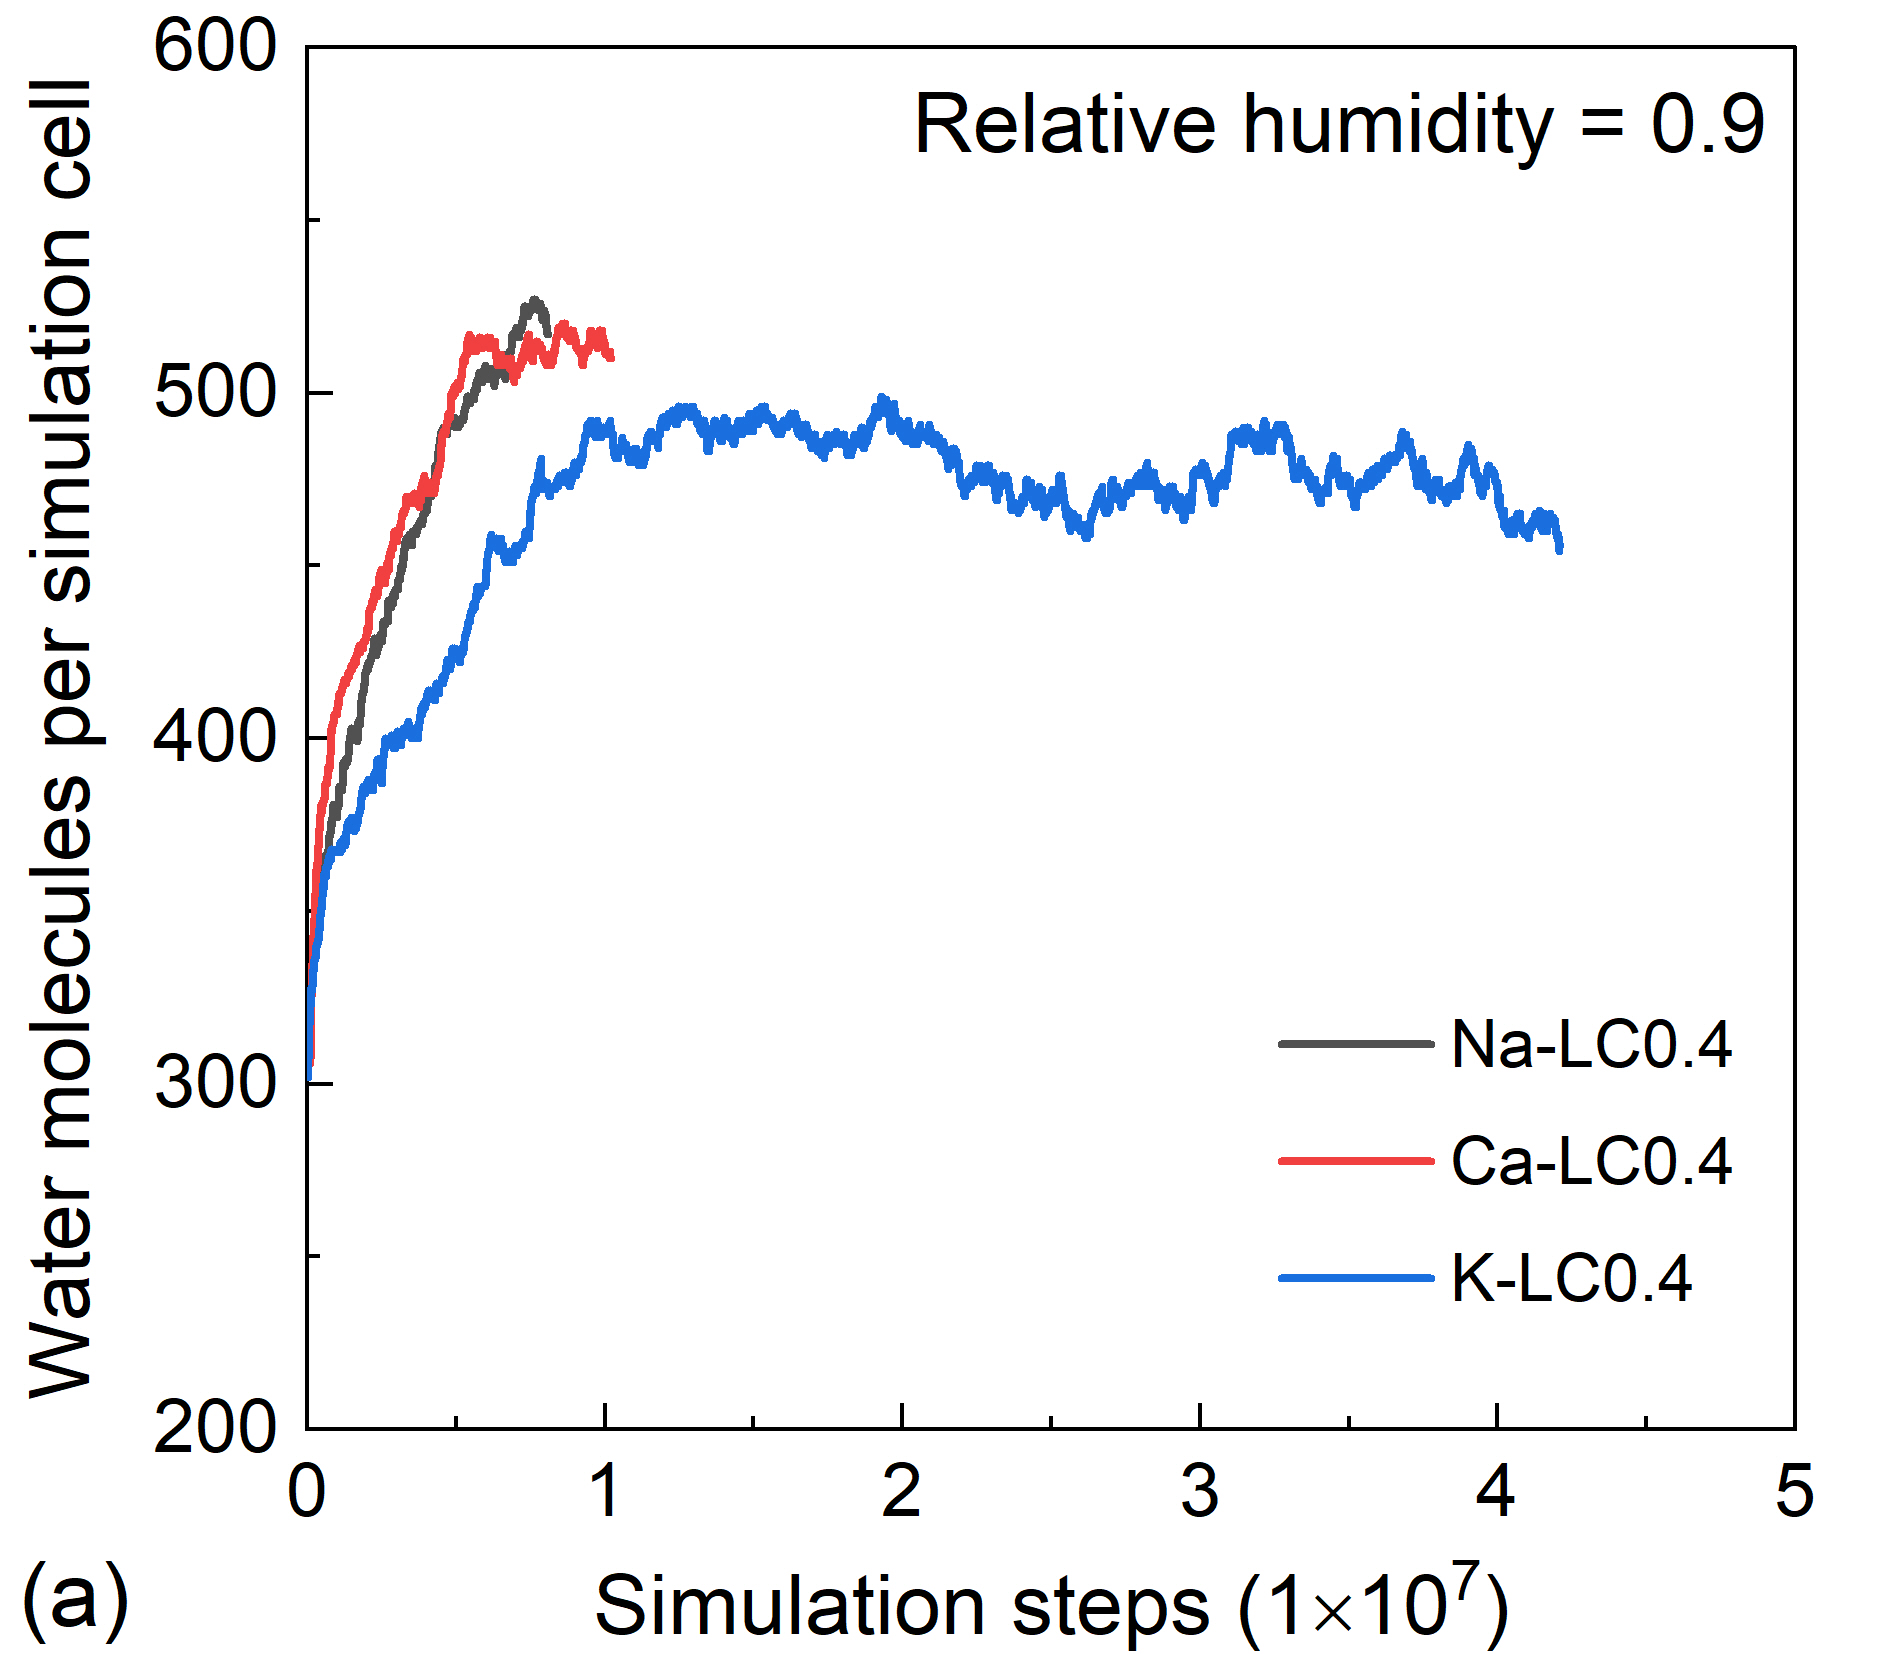
\includegraphics[width=\linewidth]{../figures/Fig6a.jpg}
    \caption{}
    \label{fig:cation_hydration_trajectories_a}
  \end{subfigure}\hfill
  \begin{subfigure}[b]{0.48\linewidth}
    \centering
    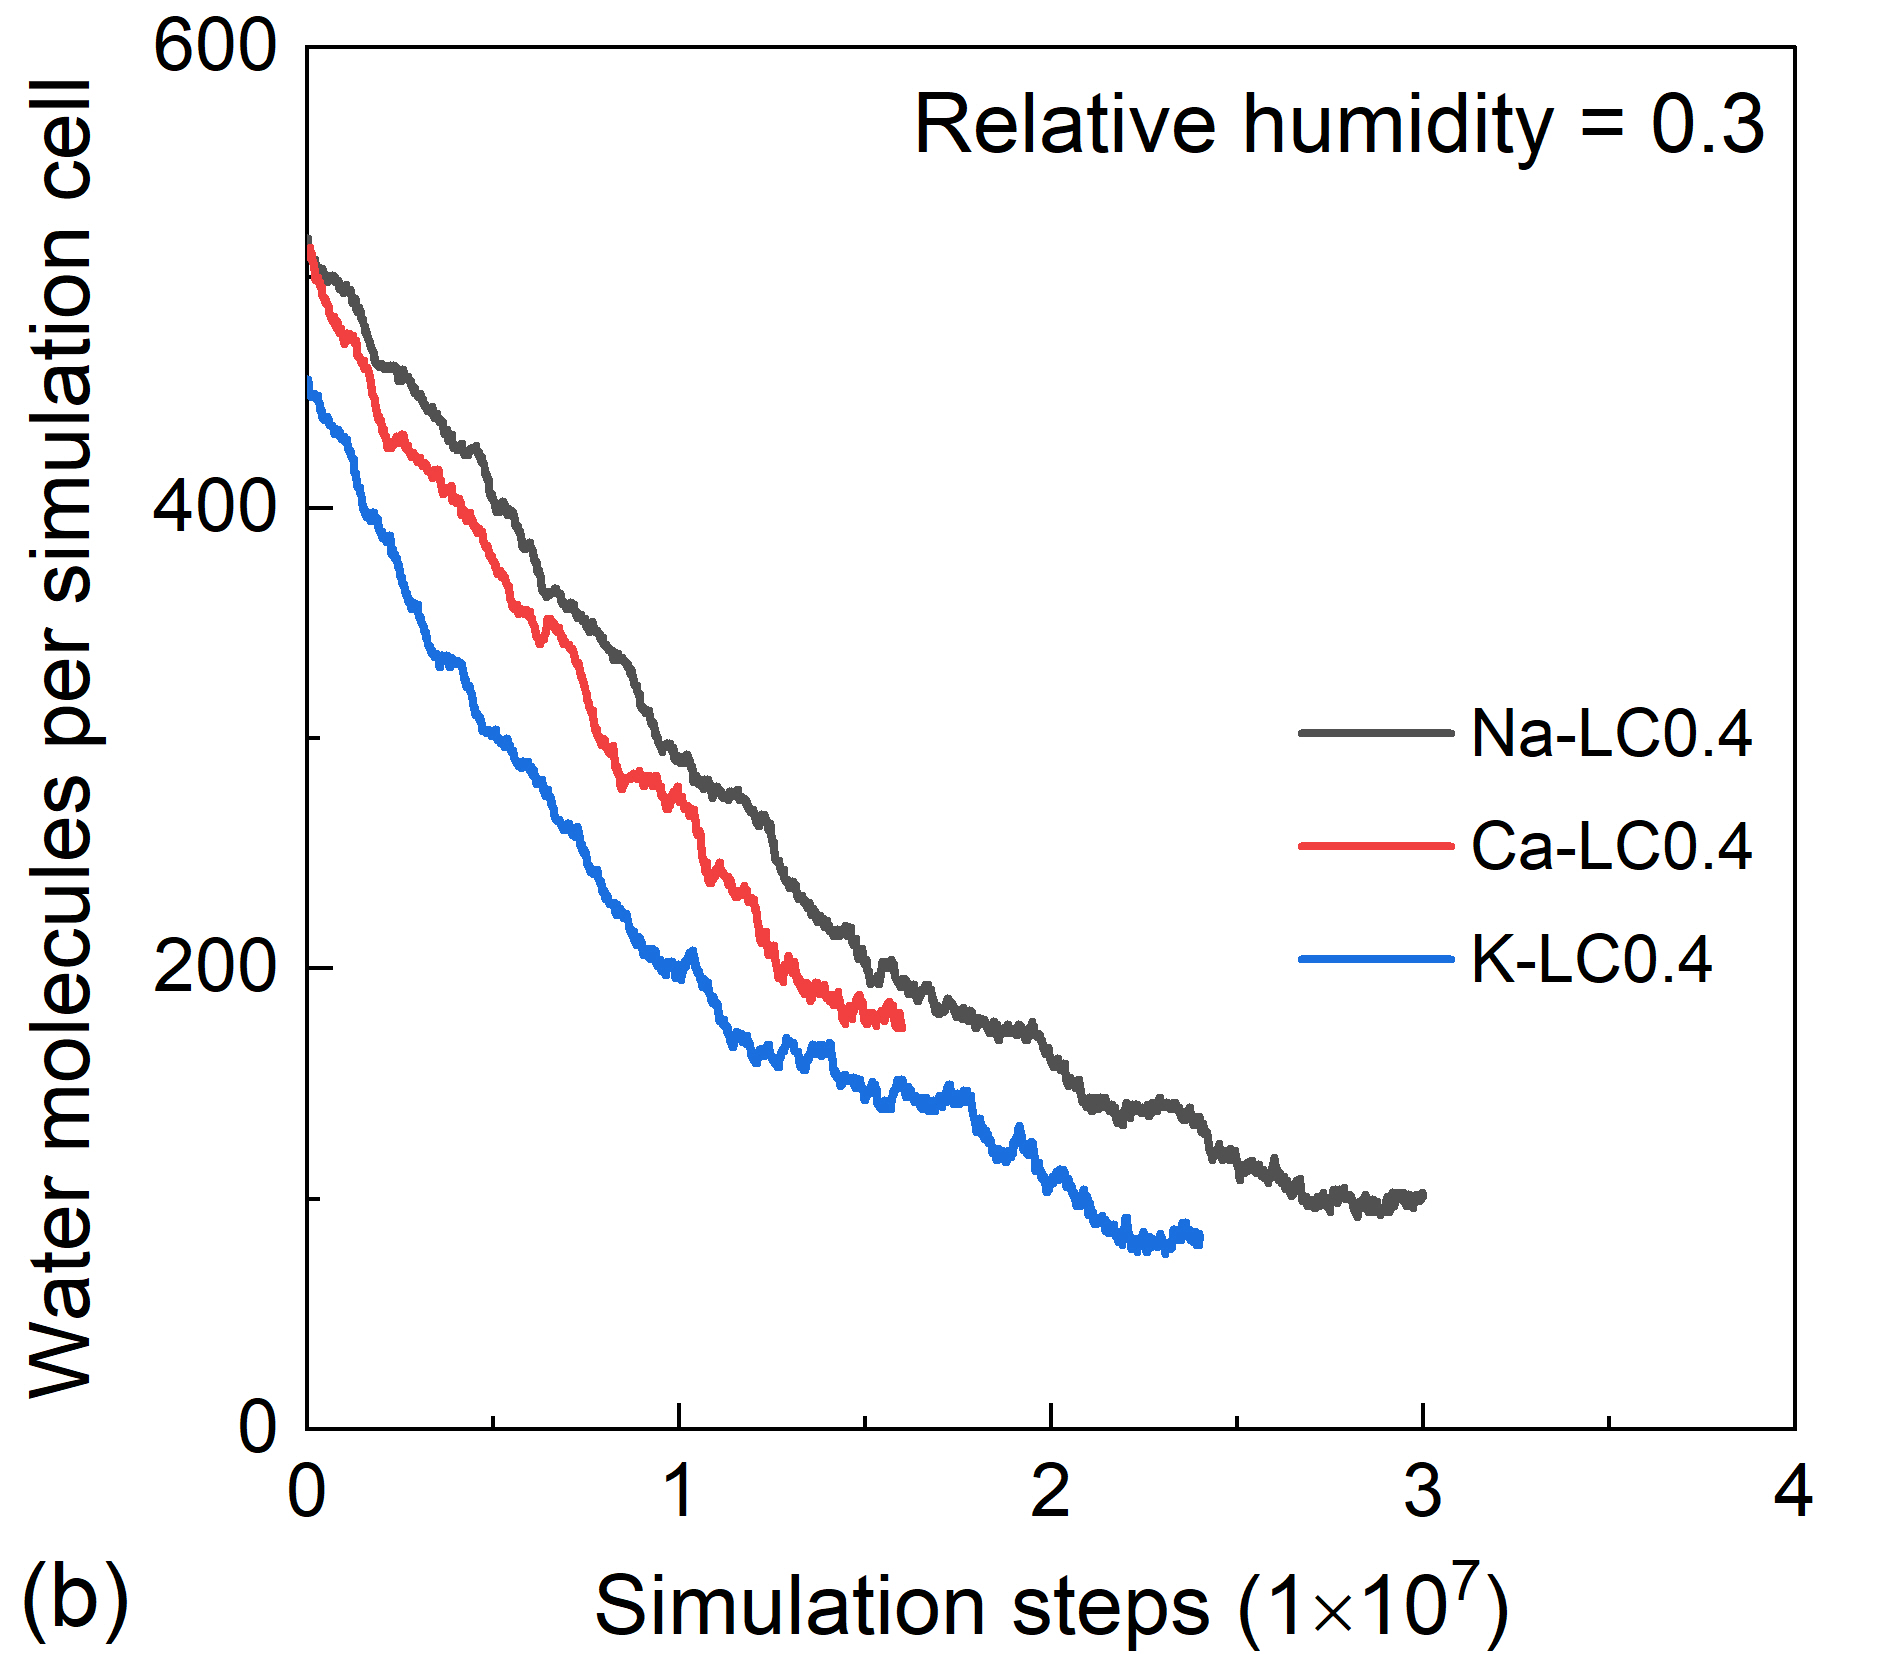
\includegraphics[width=\linewidth]{../figures/Fig6b.jpg}
    \caption{}
    \label{fig:cation_hydration_trajectories_b}
  \end{subfigure}

  \medskip
  \begin{subfigure}[b]{0.48\linewidth}
    \centering
    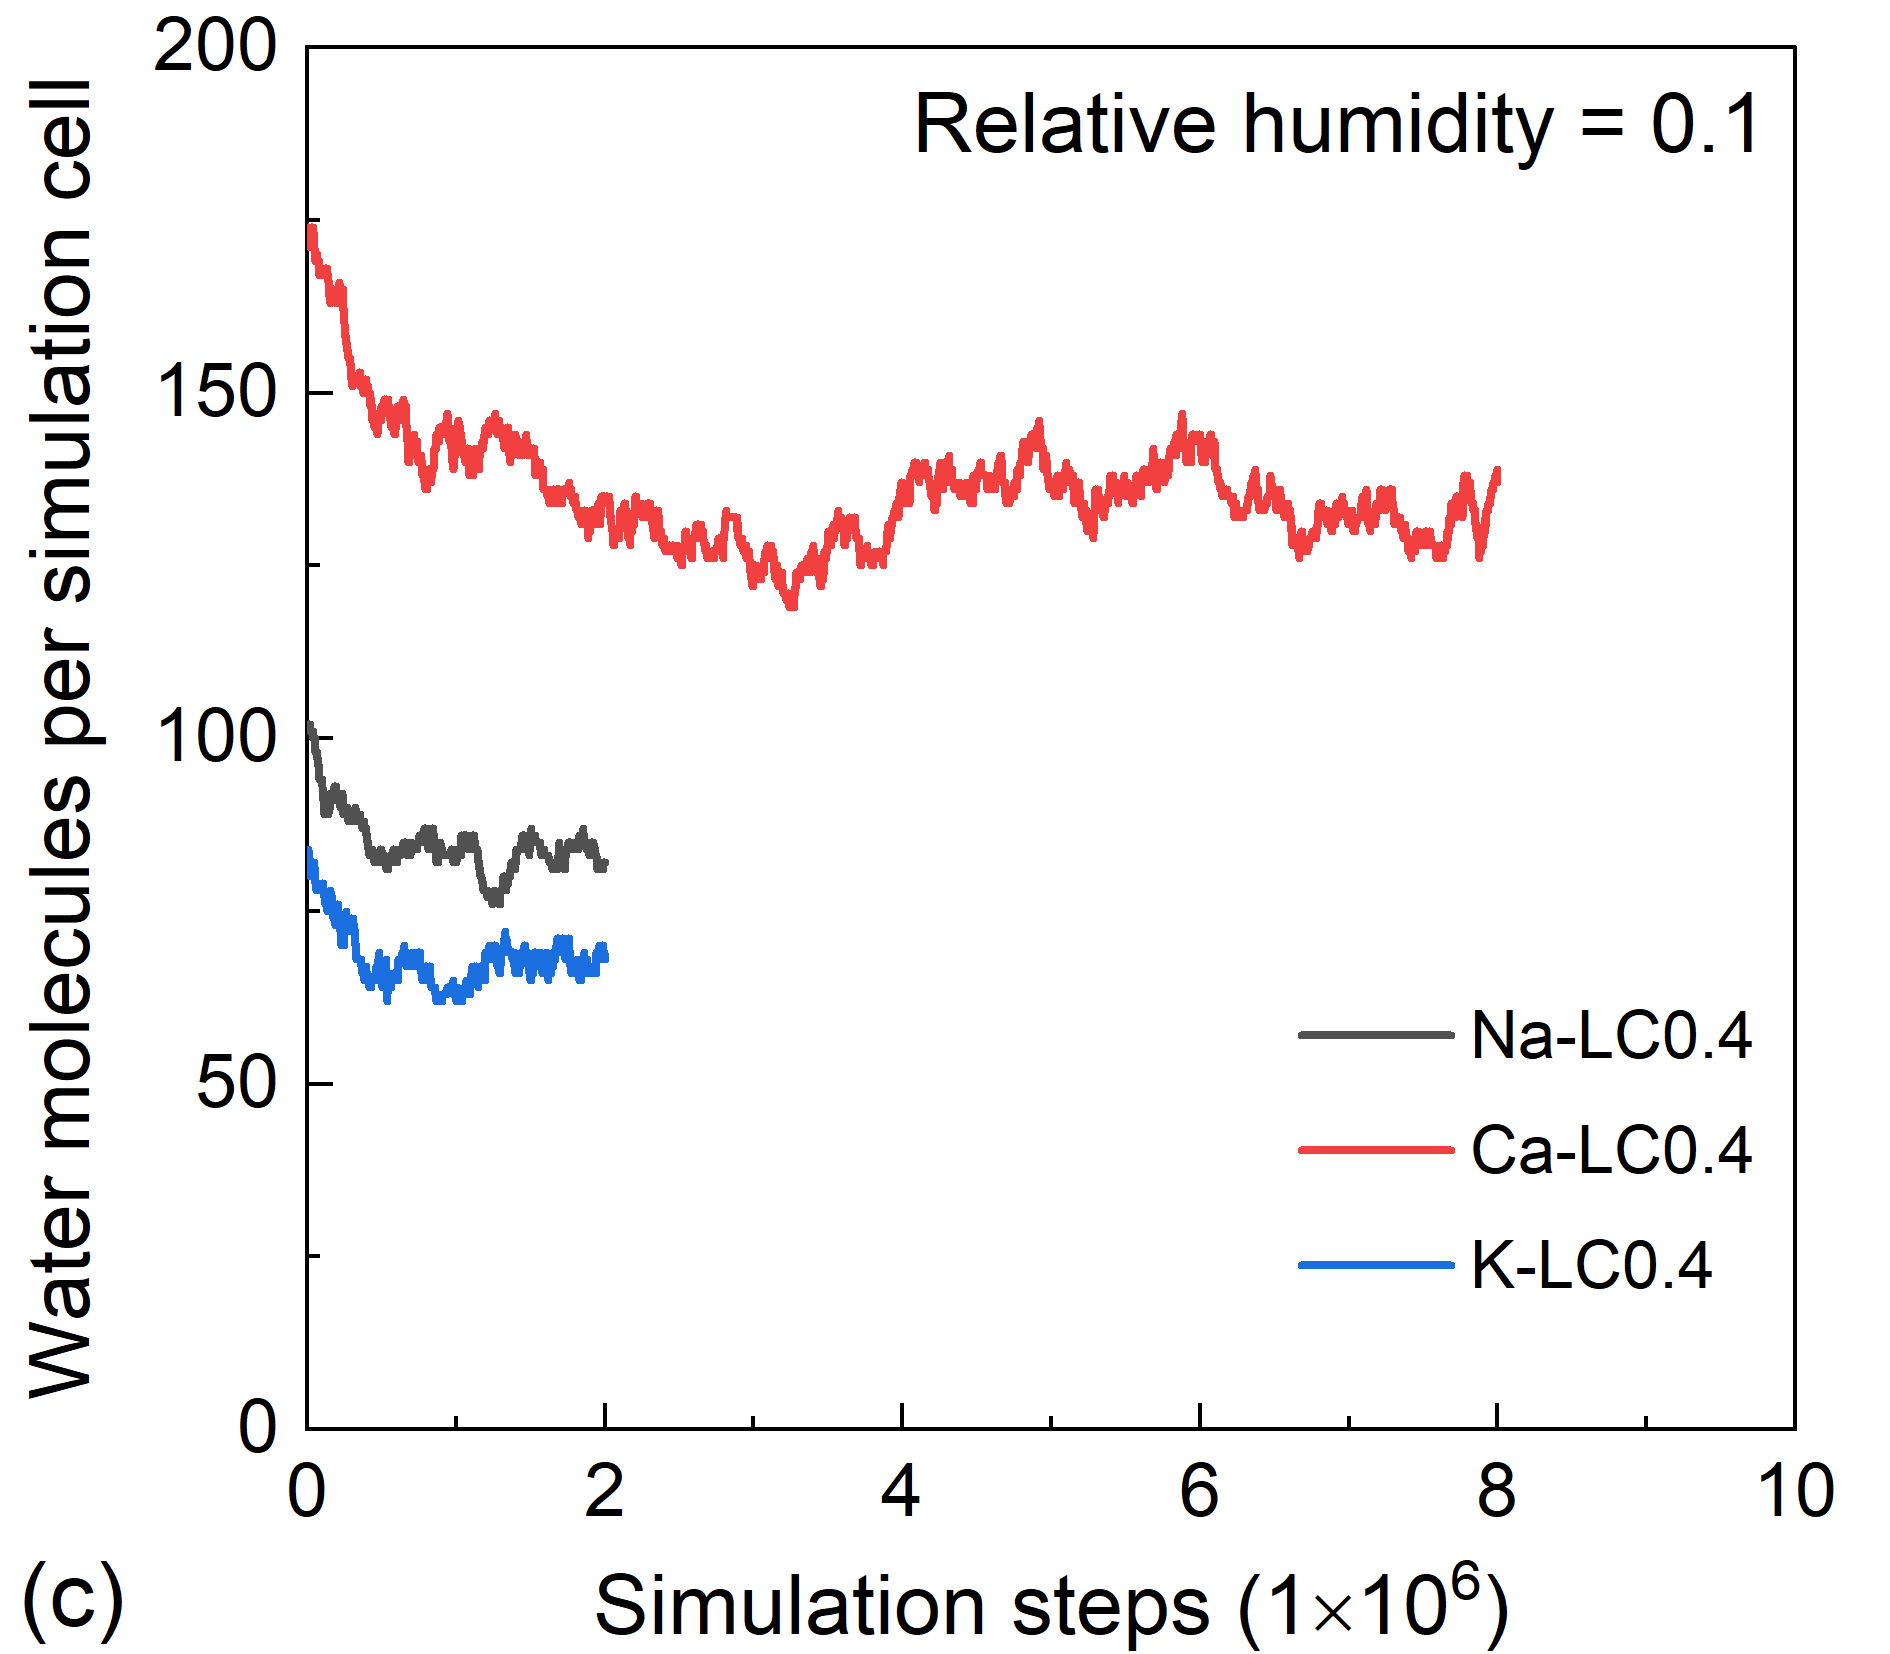
\includegraphics[width=\linewidth]{../figures/Fig6c.jpg}
    \caption{}
    \label{fig:cation_hydration_trajectories_c}
  \end{subfigure}
  \caption{Cation-dependent RH-local hydration trajectories.}
  \label{fig:cation_hydration_trajectories}
\end{figure}
\FloatBarrier

The Na-bearing systems likewise exhibited layer-charge-dependent state evolution (Figure~\ref{fig:layer_charge_hydration_trajectories}). Increasing layer charge altered both the trajectory followed during desorption and the final hydration level, with Na-LC0.5 retaining substantially more water than the lower-charge Na systems at intermediate and low RH. Layer charge therefore regulates hydration capacity and dehydration behavior by modifying the electrostatic environment experienced by interlayer water and exchangeable ions.\cite{tambach2004swelling,yang2019layercharge}

\begin{figure}[t]
  \centering
  \begin{subfigure}[b]{0.48\linewidth}
    \centering
    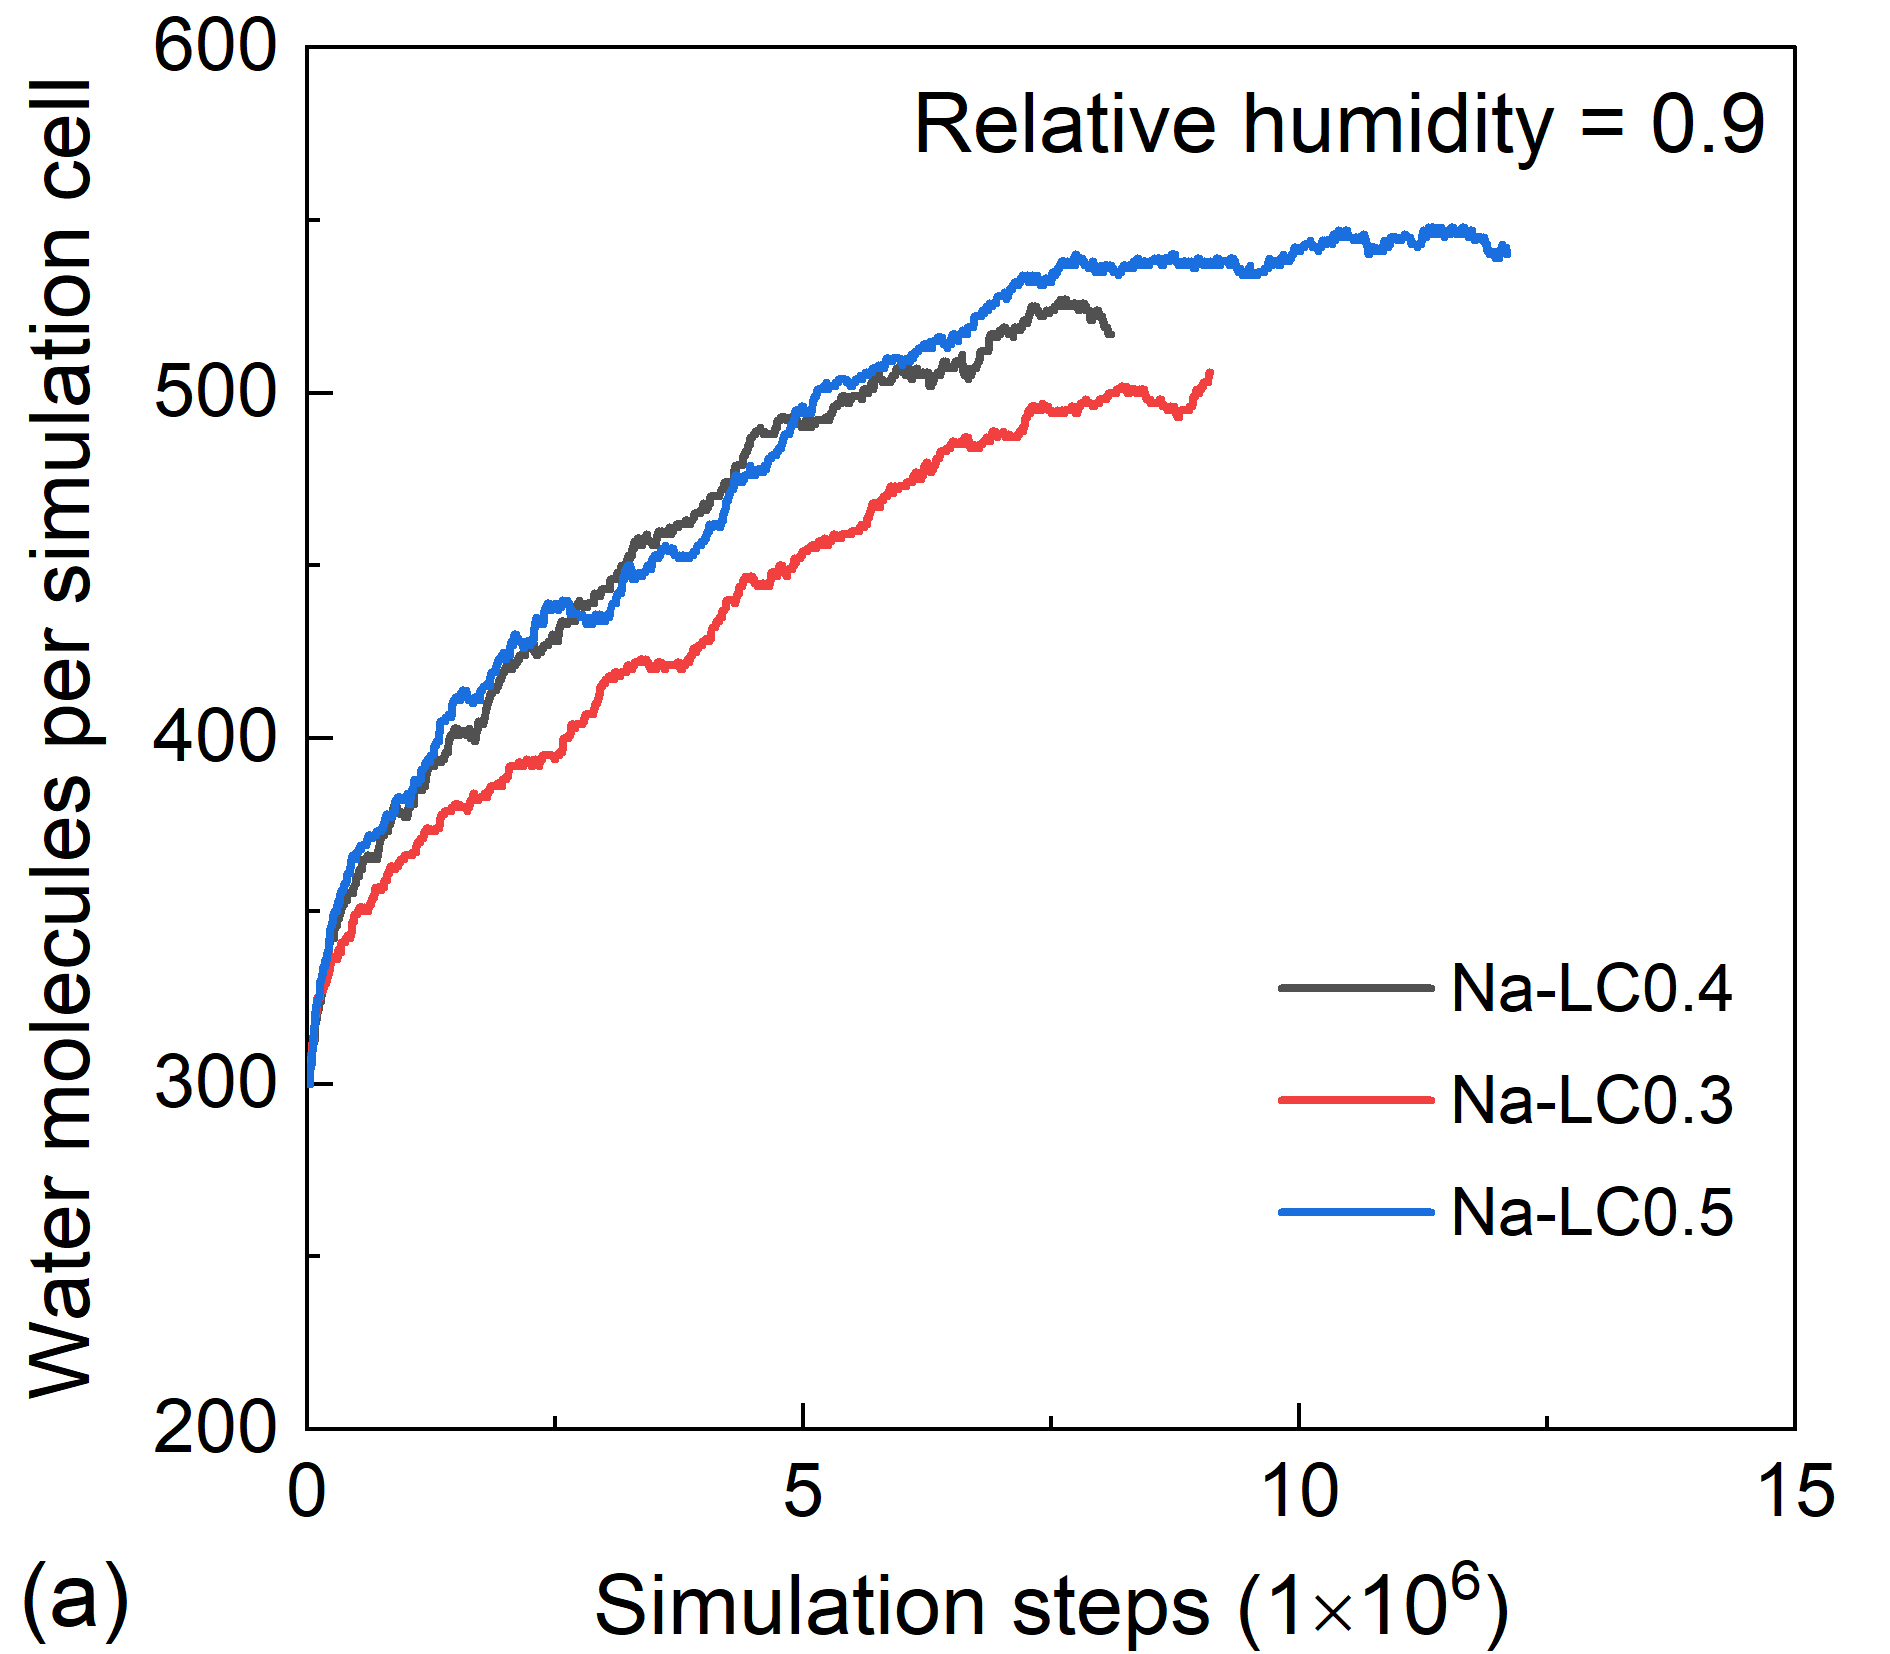
\includegraphics[width=\linewidth]{../figures/Fig7a.jpg}
    \caption{}
    \label{fig:layer_charge_hydration_trajectories_a}
  \end{subfigure}\hfill
  \begin{subfigure}[b]{0.48\linewidth}
    \centering
    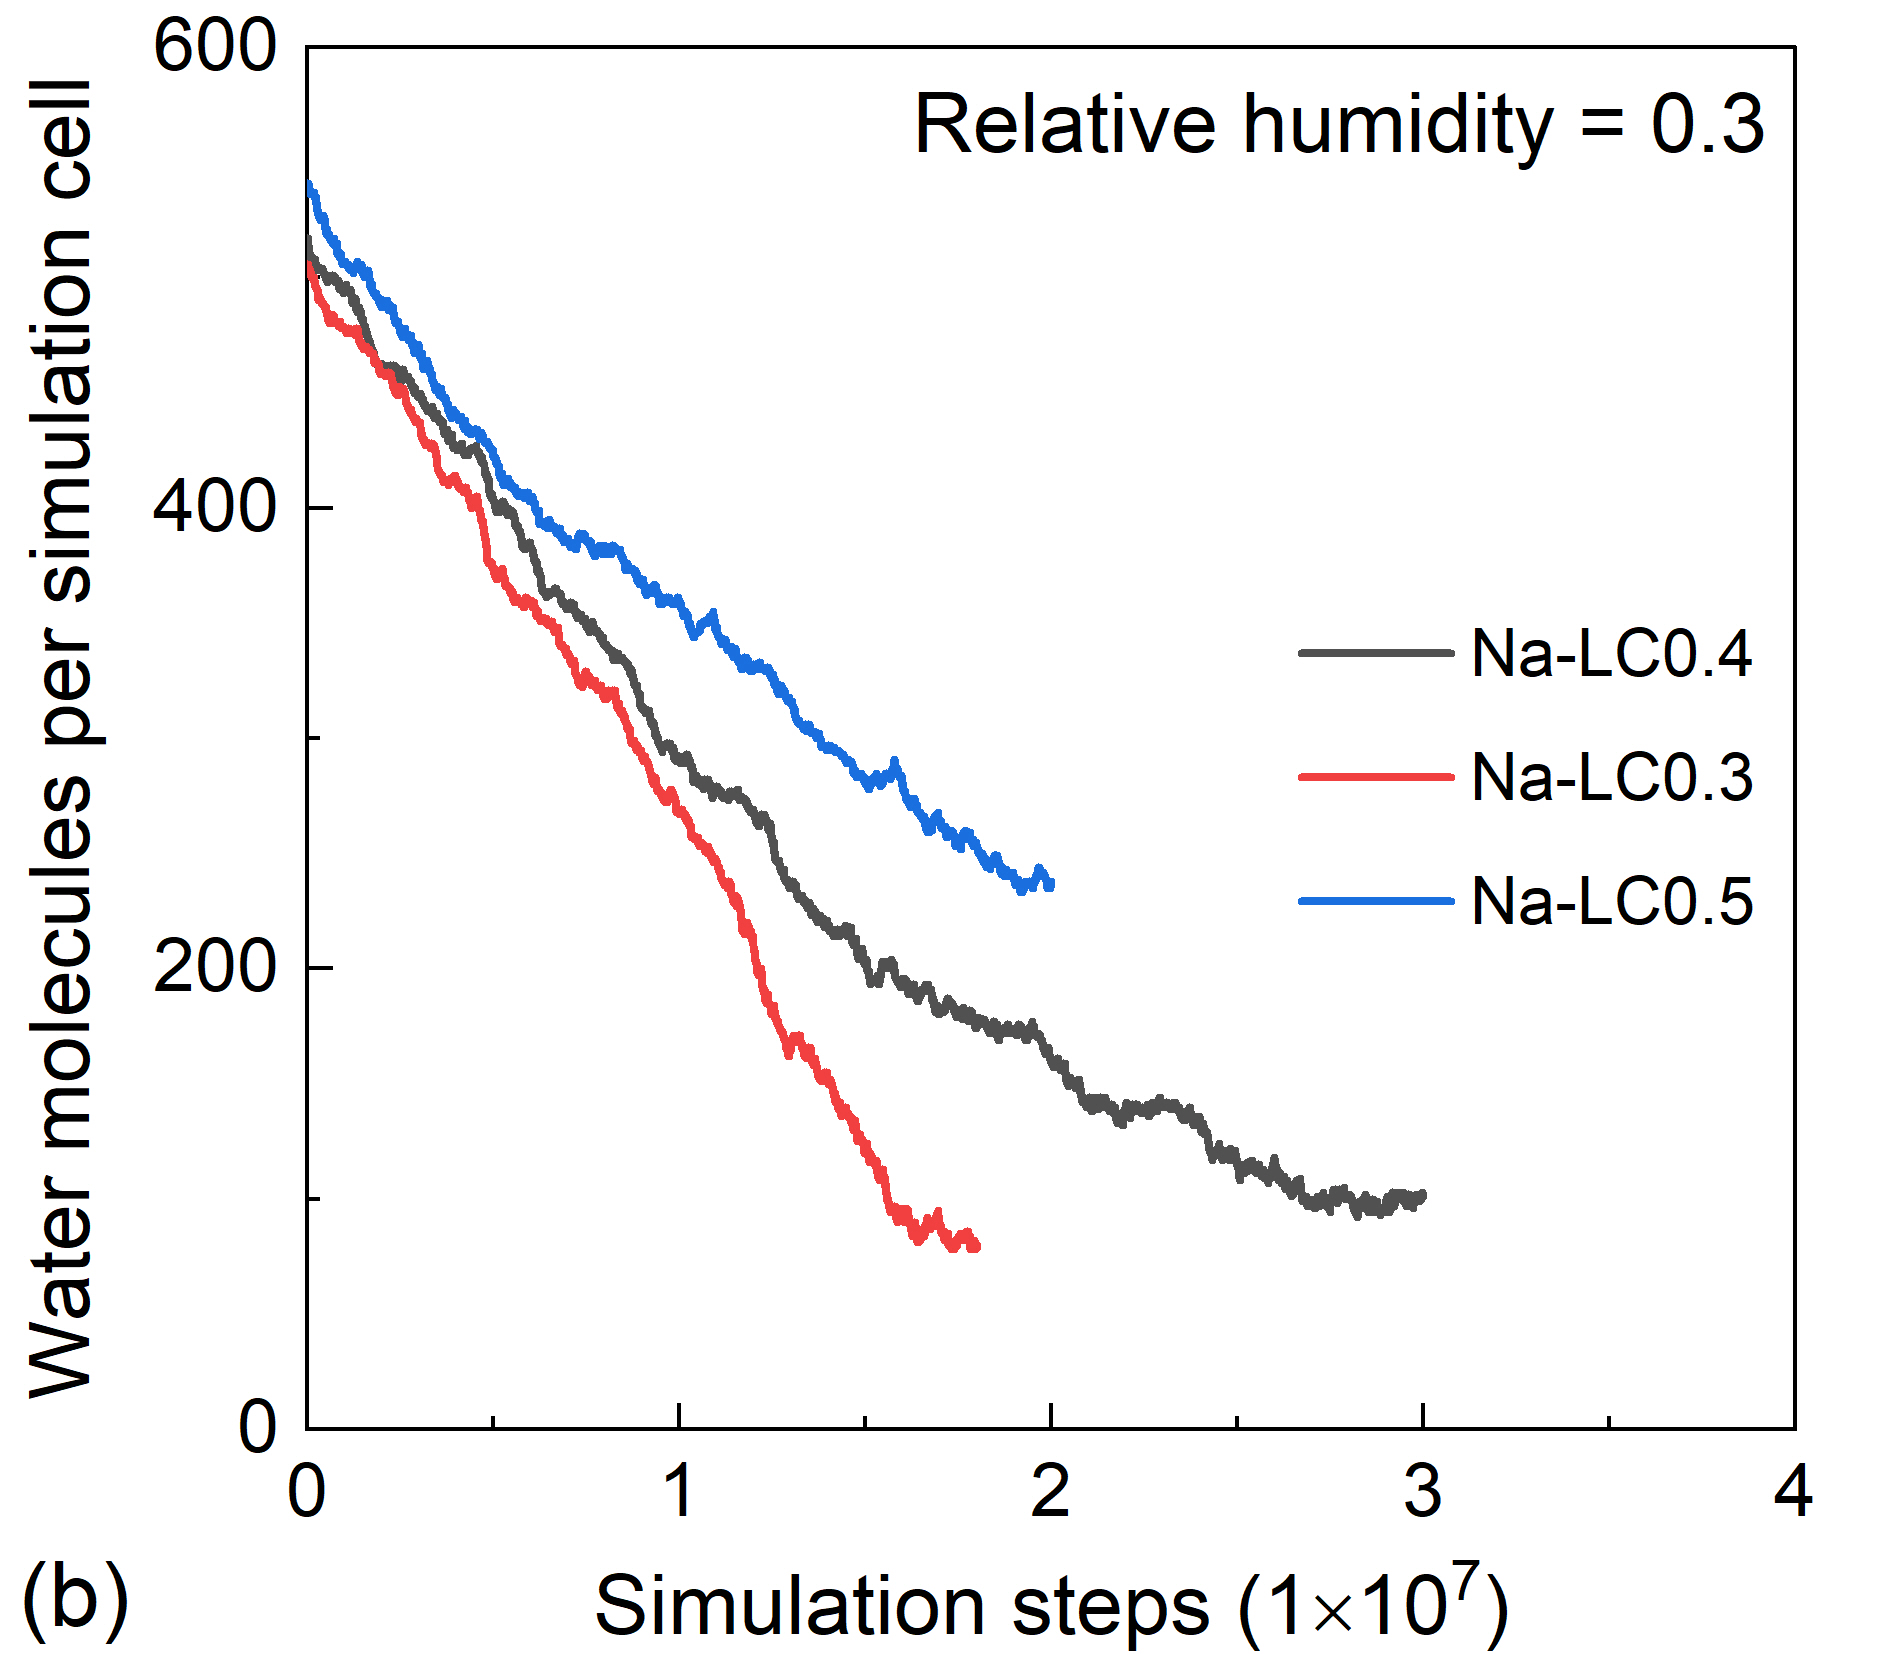
\includegraphics[width=\linewidth]{../figures/Fig7b.jpg}
    \caption{}
    \label{fig:layer_charge_hydration_trajectories_b}
  \end{subfigure}

  \medskip
  \begin{subfigure}[b]{0.48\linewidth}
    \centering
    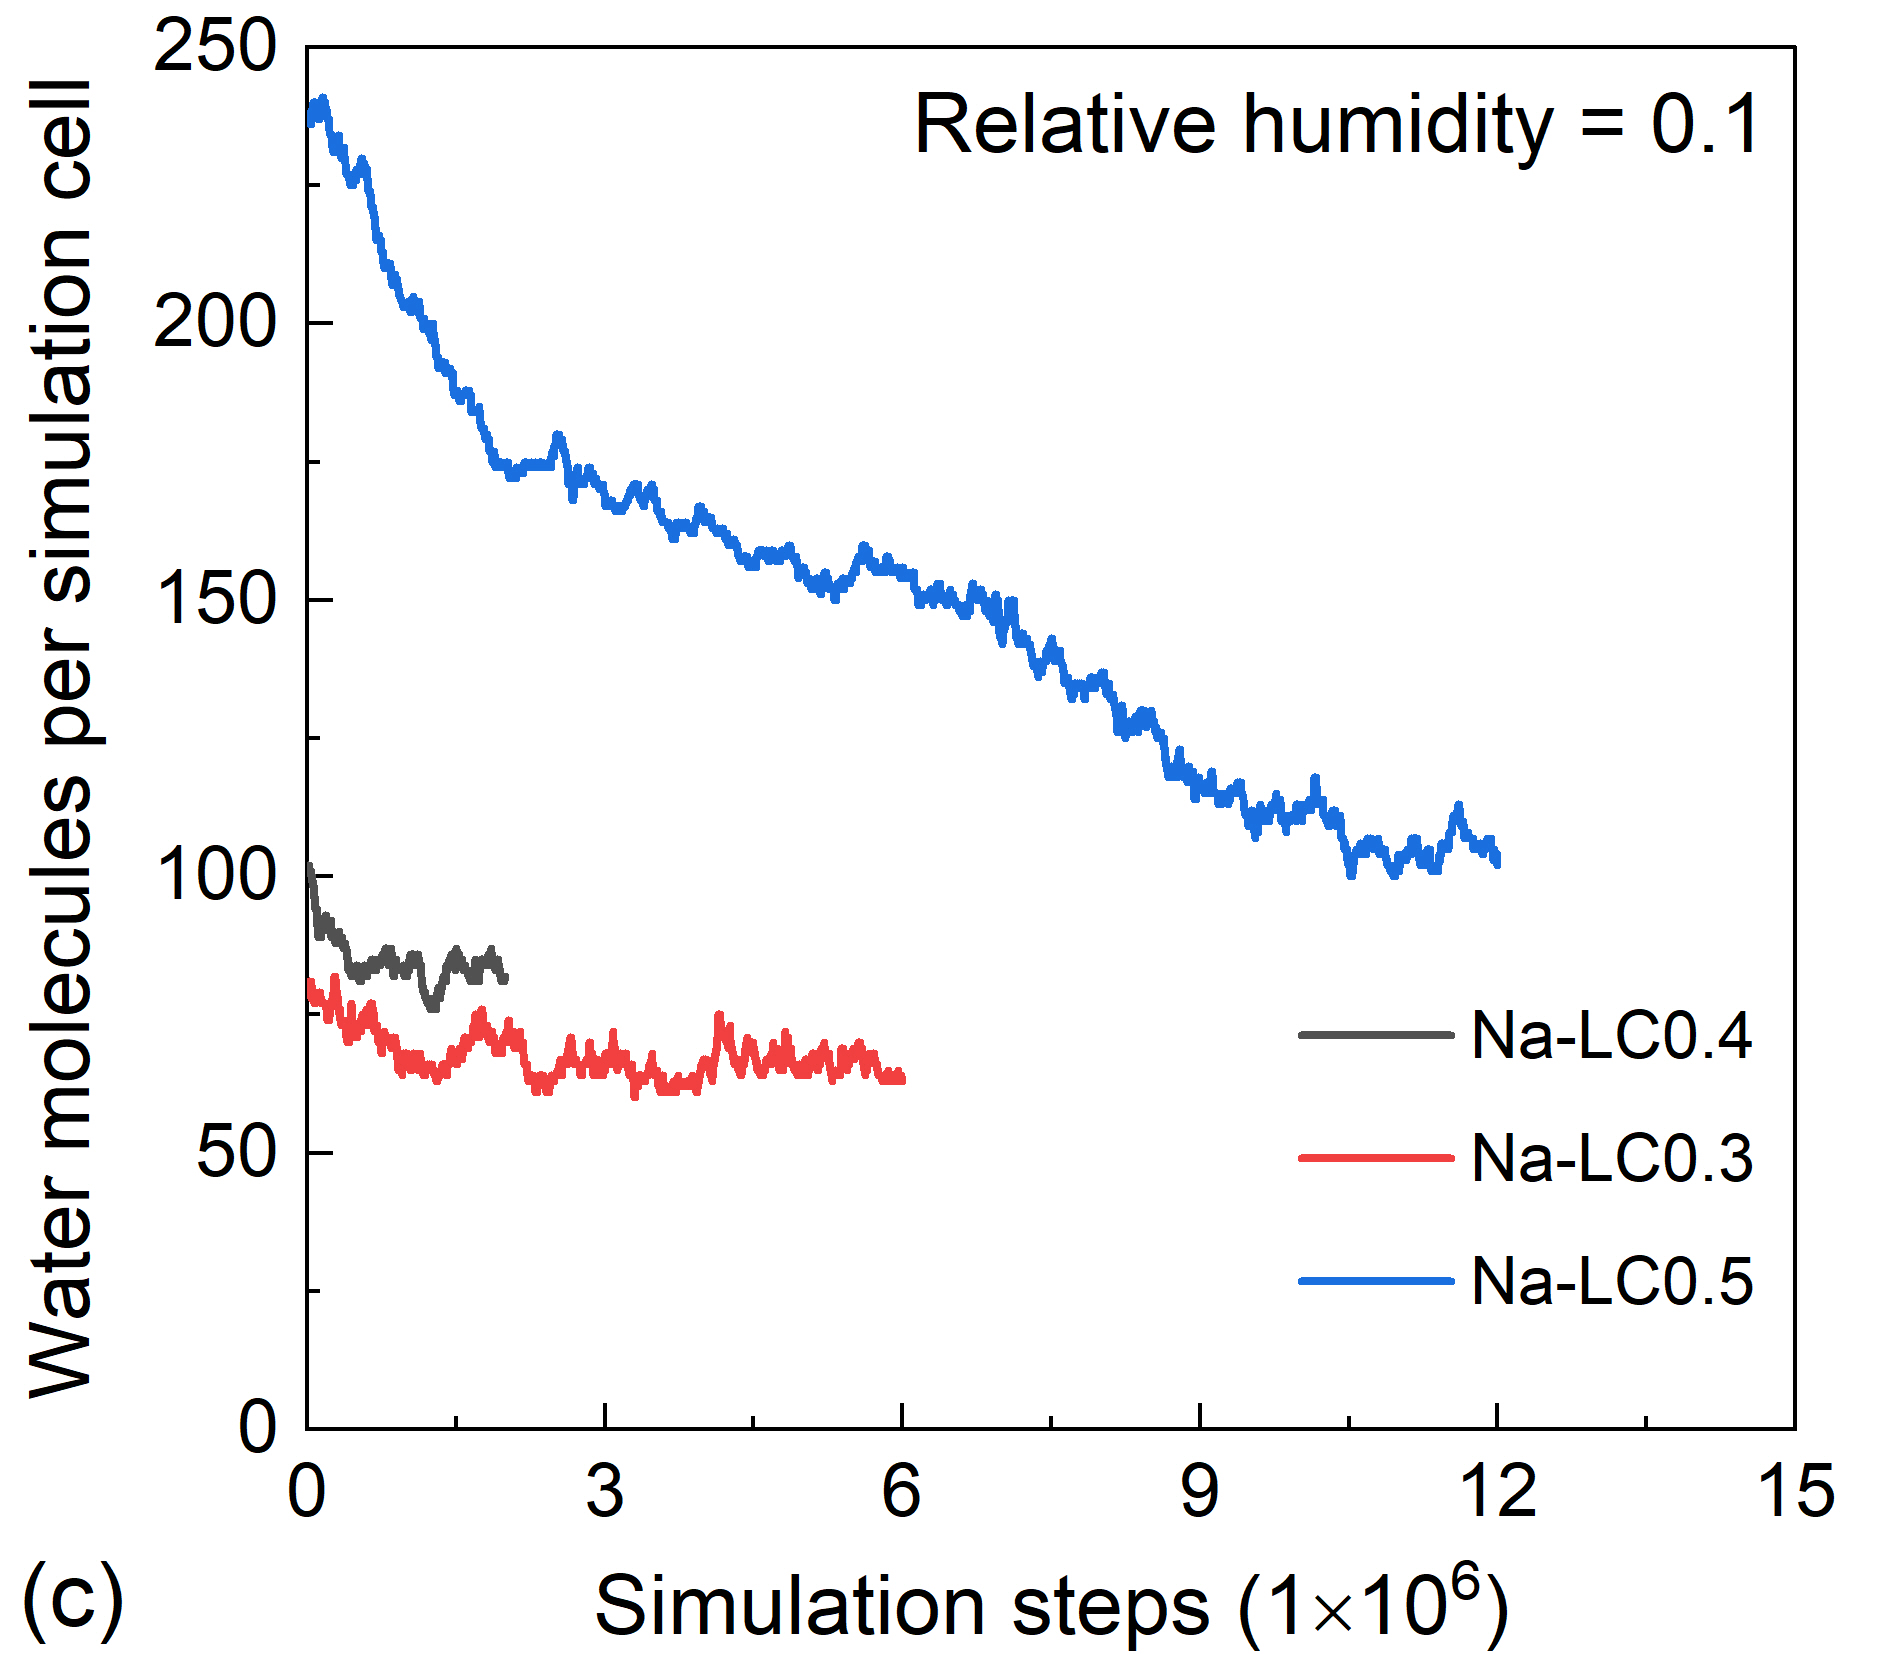
\includegraphics[width=\linewidth]{../figures/Fig7c.jpg}
    \caption{}
    \label{fig:layer_charge_hydration_trajectories_c}
  \end{subfigure}
  \caption{Layer-charge-dependent RH-local hydration trajectories.}
  \label{fig:layer_charge_hydration_trajectories}
\end{figure}
\FloatBarrier

The accepted endpoints provide a systematic comparison of equilibrium water retention across the campaign (Figure~\ref{fig:total_water_content}). Each value is a time average over the final $1.0\times10^{6}$-step production window of an accepted simulation state rather than a single configuration; the error bars are raw sample standard deviations over that window and do not represent uncertainty across independent replicas. The Ca-bearing system retained more water than the Na- and K-bearing systems at the lower RH values, while the Na and K systems showed distinct dehydration responses despite their comparable layer charge. Within the Na series, increasing layer charge increased water retention, and the separation among charge states became especially evident as RH decreased. Hydration behavior is therefore controlled by coupled effects of exchangeable-cation chemistry and layer-charge-induced electrostatic environments.

\begin{figure}[t]
  \centering
  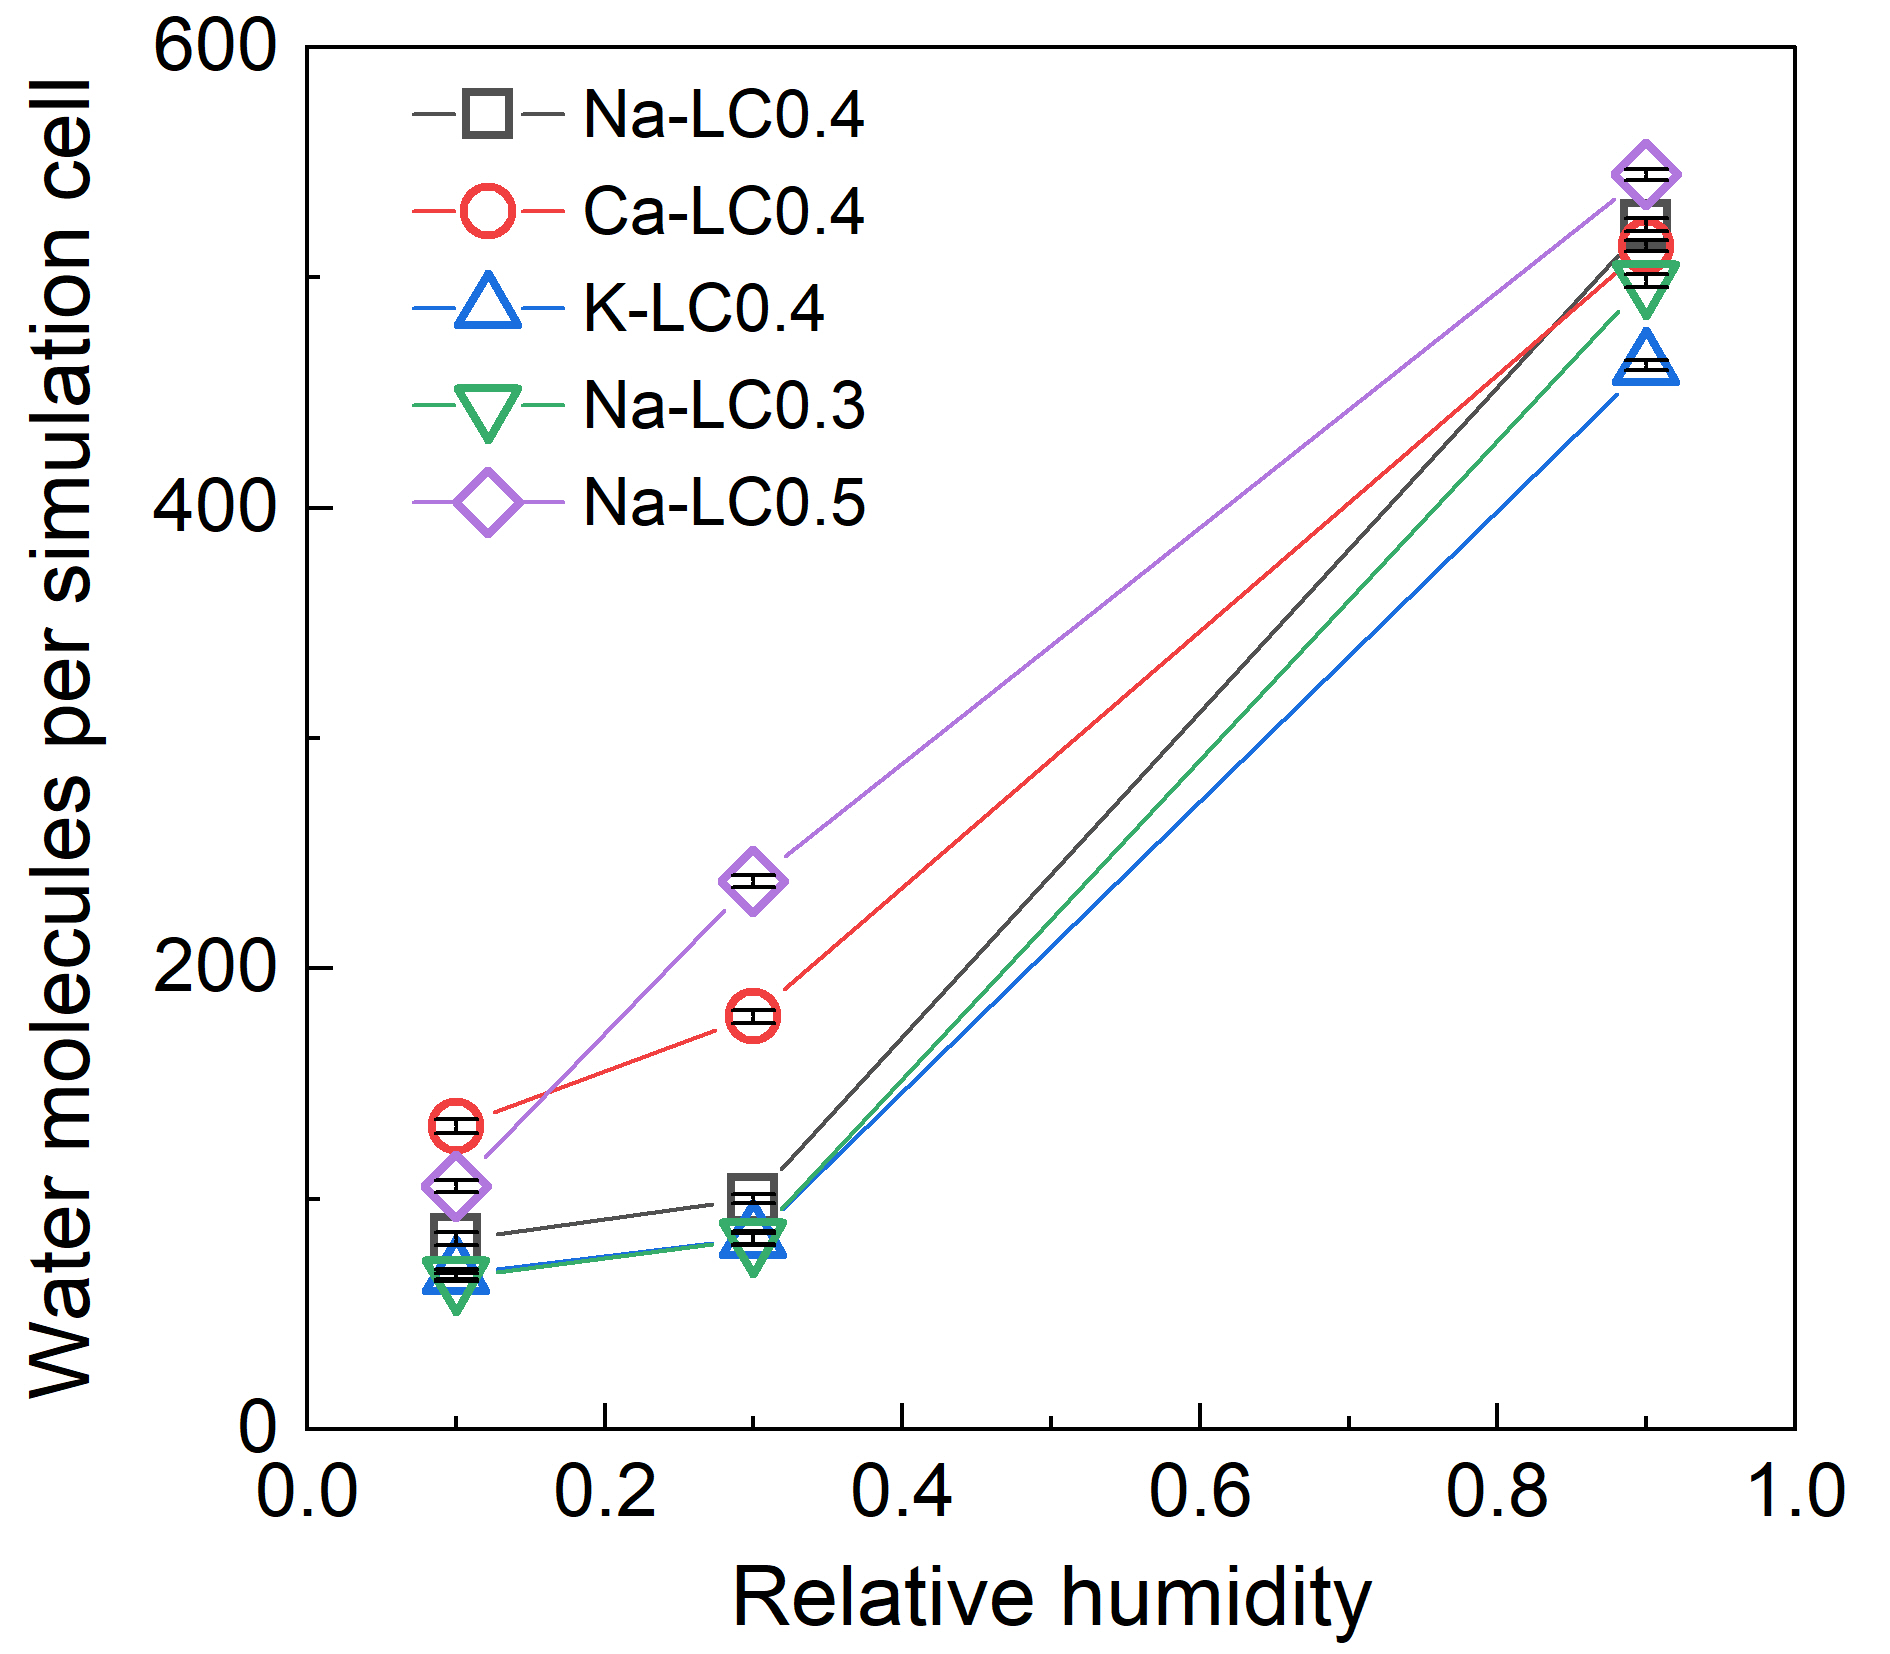
\includegraphics[width=0.95\linewidth]{../figures/Fig3.jpg}
  \caption{Total water content after RH-dependent desorption.}
  \label{fig:total_water_content}
\end{figure}
\FloatBarrier

Total water loss did not occur uniformly between spatial regions. Figure~\ref{fig:water_partitioning} separates the accepted water population into interlayer and external-surface contributions, reported per simulation cell for the common clay supercell dimensions. Interlayer water constituted a substantial fraction of the retained population throughout the campaign and was particularly persistent for the higher-charge Na system at intermediate RH. At low RH, the comparable interlayer and external populations in several systems show that dehydration redistributes the remaining water rather than removing both populations in a fixed proportion. The partitioning response thus resolves differences that are not apparent from total water alone and shows how cation chemistry and layer charge alter where water remains during dehydration.

\begin{figure}[t]
  \centering
  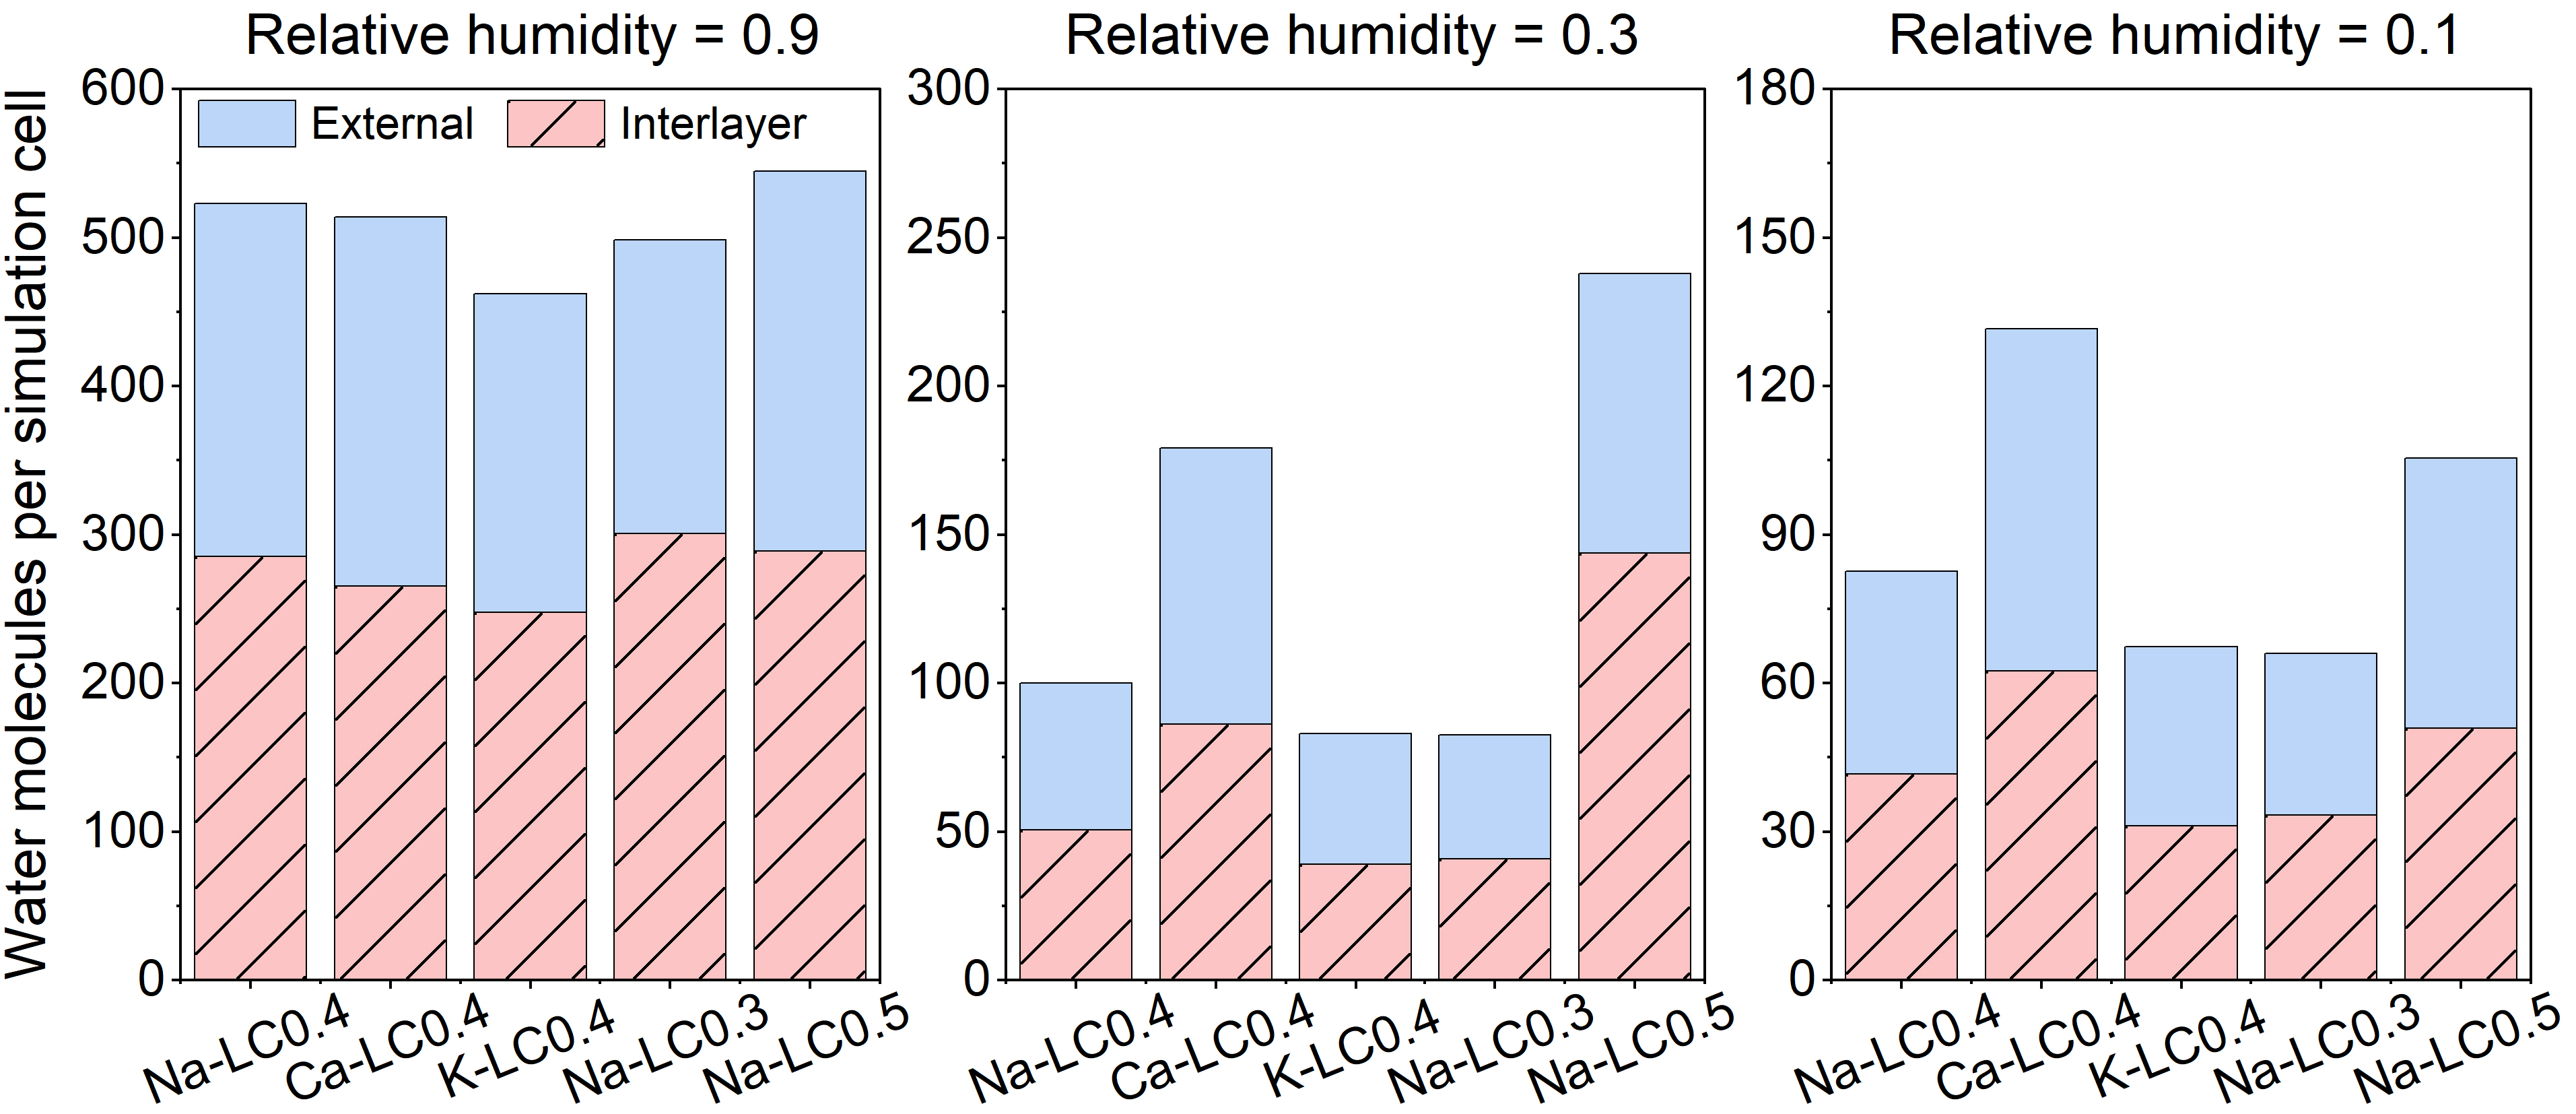
\includegraphics[width=0.95\linewidth]{../figures/Fig4.jpg}
  \caption{Water partitioning between interlayer and external regions.}
  \label{fig:water_partitioning}
\end{figure}
\FloatBarrier

The structural response follows the hydration changes (Figure~\ref{fig:basal_spacing_evolution}). Systems that retained more interlayer water generally maintained larger basal spacings: the higher-charge Na system preserved an expanded spacing at intermediate RH, and the Ca-bearing system remained more expanded than the corresponding Na- and K-bearing systems at low RH. The relationship is not strictly monotonic across all systems because basal spacing reflects the organization of confined water and ions as well as the total water population.\cite{teichmcgoldrick2015swelling,yang2019layercharge} The hydration-state assignments are therefore descriptive rather than definitive, but the combined water-partition and spacing responses demonstrate coupling between hydration state and layer configuration. Cation chemistry and layer charge jointly regulate water retention, water distribution, and structural response during dehydration.

\begin{figure}[t]
  \centering
  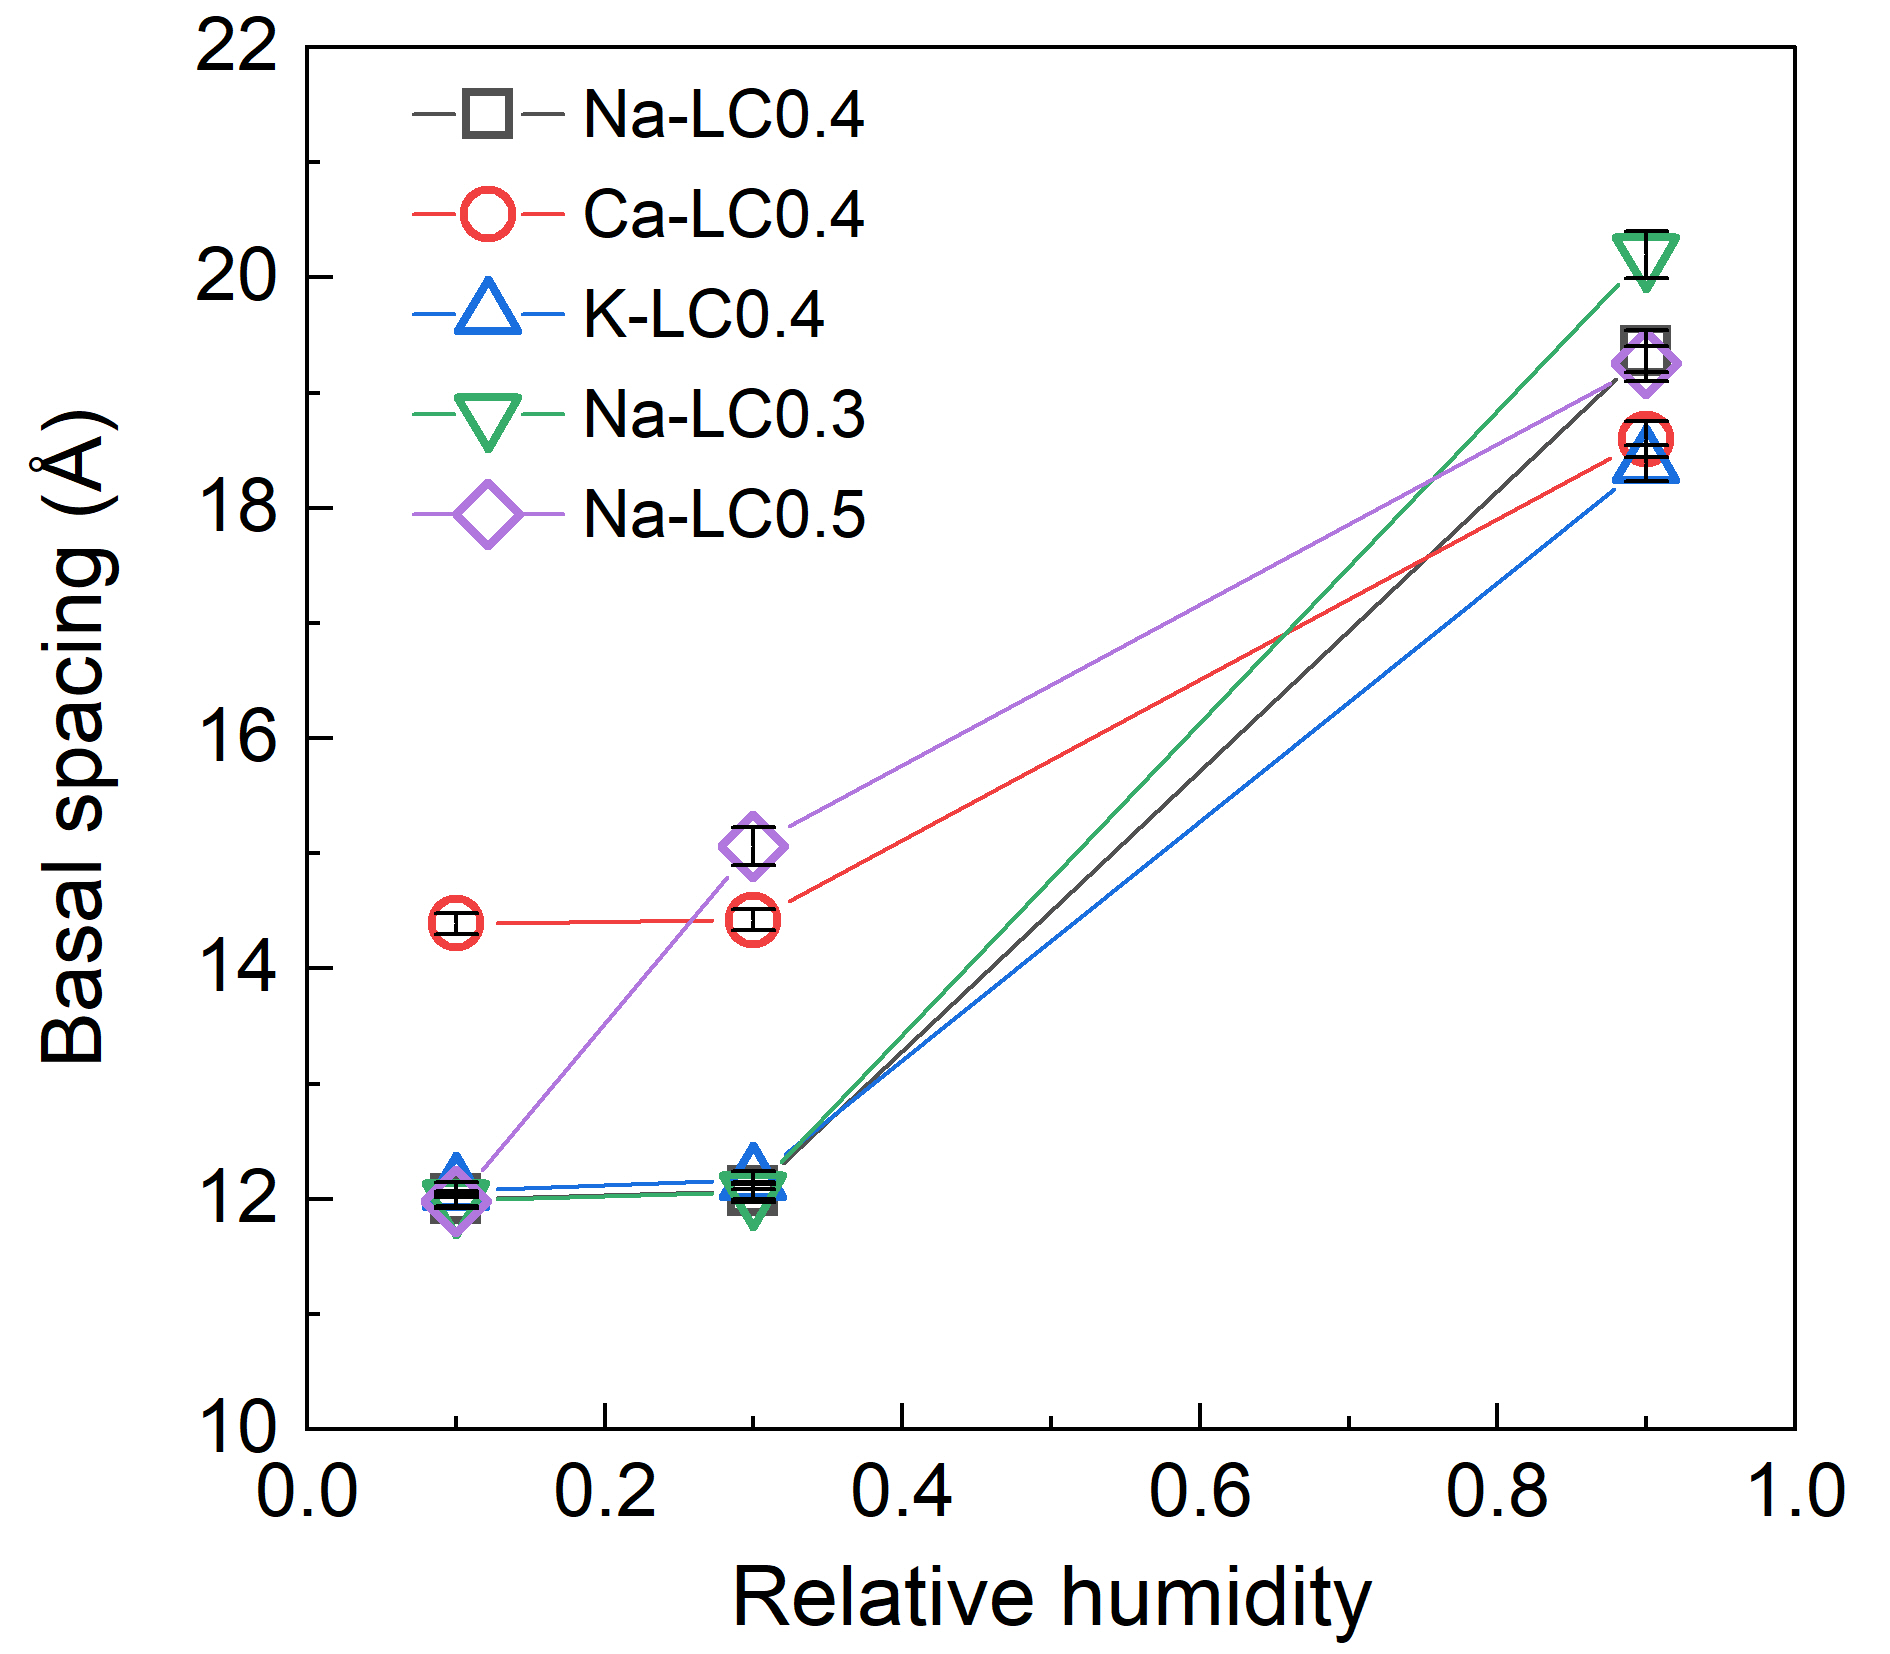
\includegraphics[width=0.95\linewidth]{../figures/Fig5.jpg}
  \caption{Basal-spacing evolution during desorption.}
  \label{fig:basal_spacing_evolution}
\end{figure}

\FloatBarrier

\subsection{Rule-Based Production and Selective Review}

Completion of the 15-state campaign establishes that the workflow operated successfully, but it does not by itself show how control was distributed between the rule-based campaign agent, scientific tools, and reasoning-agent-assisted review. We therefore reconstructed an operational census from the persistent campaign state, execution records, archive manifest, provenance records, and review state. The census distinguishes routine activity of the rule-based campaign agent from production states that could not be safely resolved by the approved workflow rules.

The completed production campaign involved 414 campaign-agent operations (Table~\ref{tab:operation_census}). The activity categories in Table~\ref{tab:operation_census} describe different recorded aspects of the workflow and are not mutually exclusive components of the total campaign-agent operation count. These records included 120 segmented simulation cycles and 120 corresponding analysis and progression-decision cycles. Their one-to-one correspondence shows that every completed production segment was followed by an explicit state assessment rather than by automatic continuation based only on job completion. The rule-based campaign agent also produced 15 accepted archives, performed the 10 RH transitions required to advance five systems across three prescribed states, and recorded 25 provenance checks associated with restart selection, archiving, and downstream progression.

\begin{table}[t]
\centering
\small
\caption{Operational census of the production campaign.}
\label{tab:operation_census}
\begin{tabular}{p{3.6cm}p{9.0cm}r}
\toprule
Metric & Operational definition & Count \\
\midrule
Campaign-agent operations & Routine workflow actions recorded or dispatched by the rule-based campaign agent & 414 \\
Simulation cycles & Completed segmented GCMC--MD production runs & 120 \\
Analysis--decision cycles & Post-segment analyses followed by a continuation, archive, or review decision & 120 \\
Provenance checks & Recorded validations of restart, archive, or state-transition consistency & 25 \\
Accepted states & System--RH simulation states written to the authoritative final archive & 15 \\
RH transitions & Successor RH states initialized from accepted predecessor states & 10 \\
States requiring review & Simulation states that could not be safely resolved by the approved workflow rules & 1 \\
Reasoning-agent invocations & Non-interactive invocations of the Codex CLI reasoning agent, powered by GPT-5.5, during formal production & 0 \\
\bottomrule
\end{tabular}
\end{table}

One production state required review, whereas no non-interactive reasoning-agent invocation occurred during formal production. Reasoning-agent invocation was a separate guarded action and was not automatically triggered by classification of the state as requiring review. The rule-based campaign agent nevertheless remained active throughout the campaign, while the optional Codex CLI reasoning agent, powered by GPT-5.5, remained outside routine execution. Planning interactions, software development, validation tests, and retrospective replay are excluded from the formal production reasoning-agent-invocation count.

The operational census therefore shows that long campaign duration and high action count did not require continuous LLM participation. The rule-based campaign agent and scientific tools handled the repeated simulation, analysis, archiving, provenance, and state-progression workload, while the review mechanism remained available for the small number of states that could not be safely resolved by the approved workflow rules.

\FloatBarrier

\subsection{Authentic Incidents, Blinded Replay, and Targeted Recovery}

The operational census in Section~3.2 identified one authentic production state requiring review. We examined this incident together with a preserved provenance conflict.

The production state requiring review occurred for K-LC0.4 at RH = 0.3. The accepted RH = 0.9 predecessor state ended at an absolute LAMMPS timestep of 42.1 million, after which the rule-based campaign agent stopped the RH = 0.3 simulation state at 60.1 million absolute timesteps because its budget logic evaluated the inherited counter against a limit intended for the current state. The numerical timestep counter remained valid and continuous through the restart chain, but the RH = 0.3 trajectory had accumulated only 18 million RH-local steps. The error arose because the inherited absolute timestep was used to evaluate a state-local production budget.

Recovery used corrected RH-local step accounting rather than a simple increase of the numerical limit. The rule-based campaign agent was corrected to evaluate RH-local elapsed steps and resumed the K-LC0.4 RH = 0.3 simulation state from the latest valid 60.1 million-step restart. It then continued for 6 million additional steps and reached strict-pass status at 24 million RH-local steps and 66.1 million absolute timesteps. The rule-based campaign agent then initialized the successor RH = 0.1 state from the updated accepted RH = 0.3 predecessor state and archive. The successor state reached strict-pass status after 2 million RH-local steps at 68.1 million absolute timesteps.

The stale RH = 0.7 case represented a provenance conflict rather than a physical convergence anomaly. An RH = 0.7 archive existed and carried plausible completion metadata, but it originated from an earlier smoke-chain predecessor and was not part of the validated predecessor or authoritative archive chain used for final reporting. File existence, modification recency, and plausible naming were therefore insufficient evidence of authority; downstream progression had to rely on the validated archive chain.

The K-LC0.4 RH = 0.3 timestep incident and the stale RH = 0.7 artifact were subsequently converted into frozen replay cases. For each replay, the original conclusion was withheld while the structured workflow state, provenance records, and associated evidence were supplied for review. The timestep case was identified as an error in applying an inherited absolute timestep to an RH-local production budget, leading to a recommendation to correct the state-local accounting before continuation. The stale-artifact case was identified as a provenance conflict, and the deprecated smoke output was rejected in favor of the authoritative archive chain. Both replay outcomes reproduced the interpretations and conservative dispositions recorded during the original incident reviews.

